\documentclass{ieeetj}
\usepackage{cite}
\usepackage{amsmath,amssymb,amsfonts}
\usepackage{algorithmic}
\usepackage{graphicx,color}
\usepackage{textcomp}
\usepackage{placeins} % import float barrier functionality
\usepackage{xcolor}
\usepackage{hyperref}
\hypersetup{hidelinks=true}
\usepackage{algorithm,algorithmic}
\def\BibTeX{{\rm B\kern-.05em{\sc i\kern-.025em b}\kern-.08em
    T\kern-.1667em\lower.7ex\hbox{E}\kern-.125emX}}
\AtBeginDocument{\definecolor{tmlcncolor}{cmyk}{0.93,0.59,0.15,0.02}\definecolor{NavyBlue}{RGB}{0,86,125}}


\def\seclogo{\vspace{10pt}$<$Society logo(s) and publication title will appear here.$>$}
\renewcommand{\OJlogo}{}
\renewcommand{\seclogo}{}



% \def\OJlogo{\vspace{-4pt}$<$Society logo(s) and publication title will appear here.$>$}

\def\authorrefmark#1{\ensuremath{^{\textbf{#1}}}}

\begin{document}
% \receiveddate{XX Month, XXXX}
\reviseddate{14 March, 2025}
% \accepteddate{XX Month, XXXX}
% \publisheddate{XX Month, XXXX}
\currentdate{14 March, 2025}
% \doiinfo{XXXX.2022.1234567}

% \renewcommand{\reviseddate}[1]{}


% \markboth{}{Author {et al.}}

\title{ Exploring Methods of Optimizing User Item Recommendation Systems\\
       \large{MIE 424 Survey-Oriented Project}}

\normalsize{\author{Jiacheng (Jason) Chen \authorrefmark{1}, Max Zhang\authorrefmark{1}, Ken Kato\authorrefmark{1}, Dav Vrat Chadha\authorrefmark{1}, Punyaphat Sukcharoenchaikul\authorrefmark{1}}}
\affil{Department of Engineering Science, University of Toronto, Toronto, ON Canada}

% \affil{National Institute of Standards and Technology, Boulder, CO 80305 USA}
% \affil{Department of Physics, Colorado State University, Fort Collins, CO 80523 USA}
% \affil{Electrical Engineering Department, University of Colorado, Boulder, CO 80309 USA}
% \corresp{Corresponding author: First A. Author (email: author@ boulder.nist.gov).}
% \authornote{This paragraph of the first footnote will contain support information, including sponsor and financial support acknowledgment. For example, ``This work was supported in part by the U.S. Department of Commerce under Grant 123456.''}


% \begin{abstract}
% These instructions give you guidelines for preparing papers for IEEE Transactions 
% and Journals. Otherwise, use this document as an instruction set. The electronic file of your paper will be formatted further at IEEE. Paper titles should be written in uppercase and lowercase letters, not all uppercase. Avoid writing long formulas with subscripts in the title; short formulas that identify the elements are fine (e.g., ``Nd--Fe--B''). Do not write ``(Invited)'' in the title. Full names of authors are preferred in the author field, but are not required. Put a space between authors' initials. The abstract must be a concise yet comprehensive reflection of what is in your article. In particular, the abstract must be self-contained, without abbreviations, footnotes, or references. It should be a microcosm of the full article. The abstract must be between 150--250 words. Be sure that you adhere to these limits; otherwise, you will need to edit your abstract accordingly. The abstract must be written as one paragraph, and should not contain displayed mathematical equations or tabular material. The abstract should include three or four different keywords or phrases, as this will help readers to find it. It is important to avoid over-repetition of such phrases as this can result in a page being rejected by search engines. Ensure that your abstract reads well and is grammatically correct.
% \end{abstract}

% \begin{IEEEkeywords}
% Enter key words or phrases in alphabetical order, separated by
% commas. Using the \textit{IEEE Thesaurus} can help you find the best
% standardized keywords to fit your article. Use the \underline{\href{https://www.ieee.org/publications/services/thesaurus.html}{thesaurus
% access request form}} for free access to the \textit{IEEE Thesaurus}.
% \end{IEEEkeywords}

%\IEEEspecialpapernotice{(Invited Paper)}

\maketitle

\section{INTRODUCTION}
% \IEEEPARstart{T}{his} document is a template for \LaTeX. If you are
% reading a paper or PDF version of this document, please download the
% template from the IEEE Web site at 
% http://\discretionary{}{}{}ieeeauthorcenter.ieee.org/\discretionary{}{}{}create-your-ieee-article/\discretionary{}{}{}use-authoring-tools-and-ieee-article-templates/\discretionary{}{}{}ieee-article-templates/
% so you can use it to prepare your manuscript.
% You can also explore using the Overleaf editor at
% https://\discretionary{}{}{}www.overleaf.com/\discretionary{}{}{}blog/\discretionary{}{}{}278-how-to-use-overleaf-with-ieee-collabratec-your-quick-guide-to-getting-started\discretionary{}{}{}\#.xsVp6tpPkrKM9

% If your paper is intended for a conference, please contact your conference
% editor concerning acceptable formats for your particular
% conference.

% IEEE will do the final formatting of your paper. If your paper is intended
% for a conference, please observe the conference page limits.

\IEEEPARstart{U}{ser}-item recommendation systems are crucial in modern digital platforms, driving personalized experiences in domains such as e-commerce, streaming services, and social media. These systems leverage machine learning to predict user preferences based on historical interactions, ensuring that users receive relevant content, products, or services. However, optimizing recommendation systems remains a significant challenge due to the need for high accuracy, computational efficiency, and adaptability to evolving user behavior.

In this project, we aim to study different optimization techniques for user-item recommendation systems, focusing on methods that enhance recommendation accuracy and efficiency. Specifically, we investigate the effectiveness of Collaborative Filtering, Content-enriched recommendation, temporal models, and Deep Reinforcement Learning (DRL) in improving recommendation performance. Mathematically, all these methods are trying to optimize the following problem:

\begin{equation}
\label{eq:opt}
\begin{aligned}
	\hat{R}_{ui} = f(u, i \mid \Theta)
\end{aligned}
\end{equation}

where $\hat{R}_{ui}$ is the predicted rating for user $u$ on item $i$, $f$ is the optimization function, and $\Theta$ represents the model parameters. The goal is to minimize the prediction error between the predicted ratings and the actual ratings, typically using a loss function such as Mean Squared Error (MSE) or Mean Absolute Error (MAE).


\textcolor{red}{TODO: fix the explaining sentences by reflecting the new section separations more}

Different learning-based optimization techniques approach this problem in distinct ways. Autoencoders treat recommendation as a latent representation learning problem, compressing user-item interactions into a lower-dimensional space to extract meaningful embeddings that reveal hidden relationships. Convolutional Neural Networks (CNNs) take a spatial feature extraction approach, applying convolutional filters to structured representations of user-item interactions to capture local patterns and shared item attributes. Neural Attention Mechanisms cast recommendation as a context-aware learning problem, dynamically weighting past interactions to focus on the most relevant items and personalize recommendations. Recurrent Neural Networks (RNNs) frame recommendation as a sequential prediction problem, leveraging temporal dependencies in user behavior to anticipate future preferences. Meanwhile, Deep Reinforcement Learning (DRL) treats recommendation as a decision-making problem under uncertainty, optimizing long-term user engagement by learning policies that maximize cumulative satisfaction.

By systematically comparing these approaches, we aim to provide insights into their respective strengths, weaknesses, and practical trade-offs.

\section{Related Works and methodologies}

\subsection{Collaborative Filtering}

Collaborative Filtering (CF) builds recommendation systems by leveraging a user-item interaction matrix \( R \in \mathbb{R}^{u \times i} \), where \( u \) and \( i \) denote users and items. Traditional CF methods like matrix factorization and neighborhood models struggle to capture complex, nonlinear user-item relationships. They often suffer from high computational cost, parameter inefficiency, and limited generalization due to linear assumptions. RBM-CF, for instance, requires slow contrastive divergence training and separately models discrete ratings, increasing memory use. To address these issues, the AutoRec paper proposes a deep learning-based CF model that improves expressiveness and efficiency \cite{sedhain2015autorec}.
\subsubsection{AutoRec\cite{sedhain2015autorec}}
AutoRec is an autoencoder-based framework for collaborative filtering. At its core, it projects the partially observed user-rating vector $r^{(u)}$ or item-rating vector $r^{(i)}$ to a lower-dimensional latent space and aims to reconstruct the original vector in the output space. 
Mathematically, the method minimizes the MSE loss between the original rating vector and the re-constructed output vector as shown in equation \ref{eq:autorec}:
\begin{equation}
\label{eq:autorec}
\begin{aligned}
	\mathcal{L}(\Theta) = min \sum_{r \in S} ||r - h(r; \theta)||_2^2
\end{aligned}
\end{equation}
where $h(r;\theta)$ is the output of the autoencoder after projecting the input $r$ to the latent space and reconstructing it back to the original space. 
\begin{equation}
\label{eq:h function}
\begin{aligned}
	h(r; \theta) = f(W_2 \cdot g(W_1 \cdot r + b_1) + b_2)
\end{aligned}
\end{equation}
where $\theta = \{W_1, W_2, b_1, b_2\}$ are the parameters of the autoencoder and $f$ and $g$ are activation functions. In t
The parameters learned during this training process can then be used to predict un-observed ratings in the user-item interaction matrix. Because the we can obtain two kinds of vectors from the rating matrix(user-based and item-based) the paper proposes two variants of AutoRec: Item-based AutoRec (I-AutoRec), which models item embeddings and reconstructs user ratings, and User-based AutoRec (U-AutoRec), which models user embeddings and reconstructs item ratings. Compared to previous models, AutoRec introduces several key improvements. First, it offers more efficient training by using gradient-based backpropagation instead of the computationally expensive contrastive divergence required by RBM-CF. Second, it reduces parameter count as it does not require separate parameter estimation for different rating levels, unlike RBM-CF. Finally, AutoRec enables nonlinear representation learning through activation functions such as sigmoid, allowing it to capture more complex user-item interactions compared to traditional matrix factorization, which assumes a linear latent representation.

\textcolor{red}{TODO:move to later part}

AutoRec has several limitations. It is a relatively simple model, and while a deeper version has been tested, the performance improvements are minimal, suggesting that deeper models may require further adjustments to be effective. Additionally, AutoRec does not address the cold-start problem, making it challenging to provide recommendations for new users or items that lack prior ratings. also time series data.

\subsection{Convolutional Sequence Embedding Recommendation Model(Caser)\cite{tang2018personalized}}
Traditional recommender systems mainly model a user's general preferences based on past interactions and fail to account for sequential dependencies, where more recent interactions are stronger indicators of future behavior. Top-N sequential recommendation addresses this by predicting the next items a user will likely engage with based on their recent activity. The problem is framed as having a set of users $\mathcal{U} = \{u_1, u_2, \cdots, u_{|\mathcal{U}|}\}$ and items $\mathcal{I} = \{i_1, i_2, \cdots, i_{|\mathcal{I}|}\}$, with each user $u$ having a sequence of interactions $S^u = (S_1^u, \cdots, S_{|S^u|}^u)$, where $S_i^u \in \mathcal{I}$ over time. The goal is to recommend the top N items taking the user's recent interaction as well as their general preference into account. This is different from the conventional recommendation system which considers user behaviour as a set of items and not as a sequence of items.
In the paper, the authors pointout that the previous Markov Chain-based models that aim to tackle the above problem are not sufficient in doing so for multiple reasons. They discuss that these model successfully lern the point-level influences but are not sufficient to model union-level influences where a group of interactions taken by the user could influence the users behaviour in the future. Also, Markov-Chain-based models cannot account for skip-behaviours by users where a sequence of actions that occurred not in the immediate past could have a strong influence on the user's actions. 

To address these gaps, the authors propose Caser (Convolutional Sequence Embedding Recommendation Model), which takes advantage of Convolutional Neural Networks (CNNs) to model sequential patterns in recommendation. Caser represents a sequence of recent items as an embedding matrix of size $L\times d$ where $L$ represents the number of past items taken into consideration and $d$ is the number of latent dimensions for the items. By appling a horizontal and vertical convolutional filter to the "image" of user-item interaction, they aim to detect point-level and union-level interaction of the users as well as skip-behaviors. Additionally, it incorporates user embeddings to personalize recommendations and allows for skip behaviors, making it more flexible in comparison to traditional Markov models.

The Caser architecture(see figure \ref{fig:caser-architecture} in appendix) takes the item sequence matrix and user embedding as input and outputs a probability distribution over the items, which represents the probability of the user iteracting with the item at the timestep we are predicting for. The output of the model hence can be expressed as:
\[
\begin{aligned}
	p(S_t^u \mid S_{t-1}^u, S_{t-2}^u, \cdots, S_{t-L}^u) = \sigma(y_{S_t^u}^{(u,t)}),
\end{aligned}
\]
where $y_{S_t^u}^{(u,t)}$ is the output of the model for the item $S_t^u$ given the previous items $S_{t-1}^u, S_{t-2}^u, \cdots, S_{t-L}^u$ at time $t$ and $\sigma$ is the sigmoid function. The model is trained using a binary cross-entropy loss function, which minimizes the difference between the predicted probabilities and the actual interactions In the paper, the overall loss is written as:
\[
\begin{aligned}
	\ell = \sum_u \sum_{t \in C^u} \sum_{i \in \mathcal{D}_t^u} -\log(\sigma(y_i^{(u,t)})) + \sum_{j \neq i} -\log(1 - \sigma(y_j^{(u,t)}))
\end{aligned}
\]
where $C^u$ is the set of all items that user $u$ has interacted with and $\mathcal{D}_t^u$ is the set of all items that user $u$ has interacted with at time $t$, and beyond to account for skip behaviours. Hence $C^u=\{L+1, L+2, \cdots, |S^u|\}$ and $\mathcal{D}_t^u = \{S^u_t , S^u_{t+1} \cdots S^u_{t+T}\}$.

\subsection{Attention Networks}
% text

\subsection{Recurrent Neural Networks\cite{hidasi2015session} }
Recommender systems rely on long-term user histories to generate personalized recommendations, but in many real-world scenarios—such as e-commerce sites and media platforms—user tracking is unreliable or infeasible due to privacy concerns and short user engagement. In these cases, session-based recommendation is important, where recommendations are made based only on a user's recent interactions within a session. Existing methods, including item-to-item similarity models and Markov Chain-based approaches, are limited because they either consider only the last interaction or struggle to model long-term dependencies in user behavior. To address these shortcomings, the authors of propose a Recurrent Neural Network (RNN)-based model with Gated Recurrent Units (GRUs), which captures sequential dependencies by processing an entire session as a sequence. Unlike traditional models, GRUs dynamically update their hidden state with each user interaction, learning richer session representations. In the paper, they represent the events as a one-hot encoding of the interacted item or a weighted sum of the items the user interacted with so far. When discussing the loss function used for training the RNN, the authors point out that training the model to independently estimate the ranking of events did not yield a stable learning and hence chose a pairwise ranking objective. The RNNs were trained using two types of pairwise ranking loss functions: the Bayesian Personalized Ranking (BPR) loss and the TOP1 loss. The BPR loss is defined as:
\begin{equation}
\label{eq:bpr}
\begin{aligned}
	L_{BPR}=-\frac{1}{N_S} \cdot \sum_{j=1}^{N_S} \log\left( \sigma(\hat{r}_{s,i} - \hat{r}_{s,j}) \right)
\end{aligned}
\end{equation}
This loss function is defined for a given point at one session where $N_S$ is the sample size, $\hat{r}_{s,k}$ is the score on item k at given point of the session, $i$ is the desired item and $j$ are the negative samples. 
The TOP1 loss is defined as:
\begin{equation}
\label{eq:top1}
\begin{aligned}
	L_{TOP1} = \frac{1}{N_S} \cdot \sum_{j=1}^{N_S} \mathbb{I}\{\hat{r}_{s,j} > \hat{r}_{s,i}\}
\end{aligned}
\end{equation}
where $\mathbb{I}$ is an indicator function which they approximate using a sigmoid function. In order to forc the scores of negative samples to be around zero, the authors also add a regularization term to the loss function. The final loss function is defined as:
\begin{equation}
\label{eq:final loss}
\begin{aligned}
	L_s = \frac{1}{N_S} \cdot \sum_{j=1}^{N_S} \sigma\left(\hat{r}_{s,j} - \hat{r}_{s,i}\right) + \sigma\left(\hat{r}_{s,j}^2\right)
\end{aligned}
\end{equation}


\subsection{Deep Reinforcement Learning Frameworks\cite{zheng_drn_2018}}
Traditional news recommendation methods is formulated as an optimization problem that maximize the immediate engagement, assuming a fixed user preference. However, this approach fails to optimize long-term user engagement, as news consumption is time-sensitive and user interests evolve over time. Moreover, current recommendations influence future engagement, making only optimizing current reward suboptimal . To achieve sustained engagement over an infinite horizon, the recommendation system is better modeled as a Markov Decision Process (MDP), where the objective is to maximize cumulative future rewards. In this formulation, the state represents a user's recent reading history and current news, the action is recommending some news articles, and the reward is engagement-based metrics. The policy improvement theorem and contraction mapping of state-action value functions (Q-function) guarantee the existence and convergence of the optimal recommendation policy. However, solving this MDP exactly is intractable due to the high-dimensional state-action space, as there are infinitely many news states and infinitely many recommendation combinations. To address this, the authors propose using Deep Q-Networks (DQN) for functional approximation to compress state and action spaces, enabling generalization across unseen states. Further enhancements include Double Q-Learning (DDQN) to mitigate overestimation bias, experience replay for stable learning, activeness scores to dynamically weight user engagement, and Dueling Bandit Gradient Descent (DBGD) to refine exploration-exploitation trade-off via pairwise comparisons. 



\section{Datasets and Experiments}
\subsection{AutoRec\cite{sedhain2015autorec}}
The paper utilizes popular benchmark datasets from the collaborative filtering domain, namely Movielens (with both 1M and 10M ratings) and Netflix. The experiments involve splitting the data into 90\% for training and 10 for testing, with a further 10\% of the training set reserved for hyperparameter tuning, and repeating this process multiple times to obtain average RMSE values. They compare different model variants—item-based and user-based AutoRec—against several baseline methods such as RBM-based collaborative filtering, biased matrix factorization, and LLORMA. Moreover, they conduct experiments to examine the effects of different activation functions (linear versus non-linear) and varying numbers of hidden units, as well as exploring a deeper version of the model with multiple hidden layers.

\subsection{Caser\cite{tang2018personalized}}
The paper experiments with several publicly available datasets that capture sequential user behavior. In particular, they use datasets from MovieLens (movie ratings), Gowalla and Foursquare (location-based check-ins), and Tmall (e-commerce purchase data). These datasets differ in terms of sequential signal intensity, which the authors quantify by mining sequential association rules. For their experiments, user action sequences are divided into training, validation, and test sets, and the models are evaluated using top-N recommendation metrics such as Precision@N, Recall@N, and Mean Average Precision (MAP). The proposed convolutional sequence embedding model (Caser) is compared against a variety of baseline methods—including popularity-based, matrix factorization with Bayesian personalized ranking, and both Markov chain-based and recurrent neural network models—with further analyses performed on hyperparameter settings and the contribution of different model components.

% Caser is evaluated on MovieLens, Gowalla, Foursquare, and Tmall datasets, consistently outperforming state-of-the-art models such as Factorized personalized Markov
% chains (FPMC), Fossil, and GRU4Rec in Precision@N, Recall@N, and MAP (Mean Average Precision). Results show that horizontal filters improve sequential modeling by capturing dependencies where multiple past actions jointly influence recommendations, while vertical filters effectively model point-level patterns. Caser also has some limitations: its performance varies across datasets, it requires more computation than simpler models like FPMC, and it is sensitive to hyperparameters, making training more complex.

\subsection{RNN\cite{hidasi2015session}}
The paper evaluates its GRU-based model on two real-world datasets. One dataset, from the RecSys Challenge 2015, is composed of click-stream data from an e-commerce website collected over approximately six months. This dataset includes millions of sessions and tens of millions of click events on tens of thousands of items, with sessions of length one filtered out to focus on meaningful user behavior. The second dataset comes from a video streaming service, capturing watch events over a shorter period (just under two months) and involving a much larger catalog of videos, though similarly processed to remove anomalies such as excessively long sessions. The experiments compare the proposed model against popular baselines like item-to-item similarity methods, session-based popularity predictors, and matrix factorization techniques. Additionally, the study explores various architectural choices—such as session-parallel mini-batches, output sampling strategies, and different ranking loss functions—and examines the impact of hyperparameter tuning and network configurations on the model's performance.

% The GRU-based model is evaluated on RecSys Challenge 2015 (RSC15) and a YouTube-like VIDEO dataset, showing up to a 25\% improvement in Recall@20 compared to state-of-the-art baselines like item-KNN and Bayesian Personalized Ranking Matrix Factorization (BPR-MF). Results indicate that the model effectively captures sequential dependencies, leading to more relevant recommendations. However, it has some limitations: higher training complexity, requiring GPU acceleration for scalability; lack of content-based features, meaning it relies purely on session interactions; and difficulty in hyperparameter tuning, as ranking loss functions require extensive experimentation. Additionally, like most collaborative filtering models, it still suffers from the cold-start problem, struggling to recommend items for new users with no prior interactions.

\subsection{DRL\cite{zheng_drn_2018}}
The proposed method and its enhanced variant, Double DQN (DDQN) + all tricks, outperform all baseline methods, including Logistic Regression (LR), Factorization Machines (FM), Wide \& Deep (W\&D), and bandit-based approaches (LinUCB, HLinUCB). The DDQN model achieves the highest CTR (0.1662) and nDCG (0.4877), demonstrating the effectiveness of reinforcement learning in optimizing long-term engagement. The dueling network architecture improves user-news interaction modeling, while future reward consideration in DDQN leads to additional gains in recommendation accuracy. However, in the offline setting, incorporating user activeness and exploration does not show significant improvements due to dataset limitations, as interactions are static, preventing effective exploration. The authors note that na\"{i}ve exploration strategies like $\varepsilon$-greedy can harm recommendation accuracy, suggesting that exploration should be designed more carefully. The authors propose evaluating the model in an online setting, where user engagement evolves dynamically, allowing better assessment of exploration strategies and activeness-aware recommendations. Additionally, integrating more advanced exploration methods and personalized reward functions could further enhance long-term engagement optimization.

\section{Results and Comparison}
\subsection{Formulation Comparison}
Autorec - reconstructing user-item matrix using autoencoder while minimizing MSE

Caser - using CNN to model sequenctial dependencies and user-item interaction.
\subsection{Results comparison}

\section{Conclusion and Future work}
\vfill\pagebreak


\bibliography{source}
\bibliographystyle{IEEEtran}

\appendix
\section{Appendix}
\subsection{Autorec}
\subsubsection{Visual representation of the AutoRec model}
\begin{figure}[h]
\centering
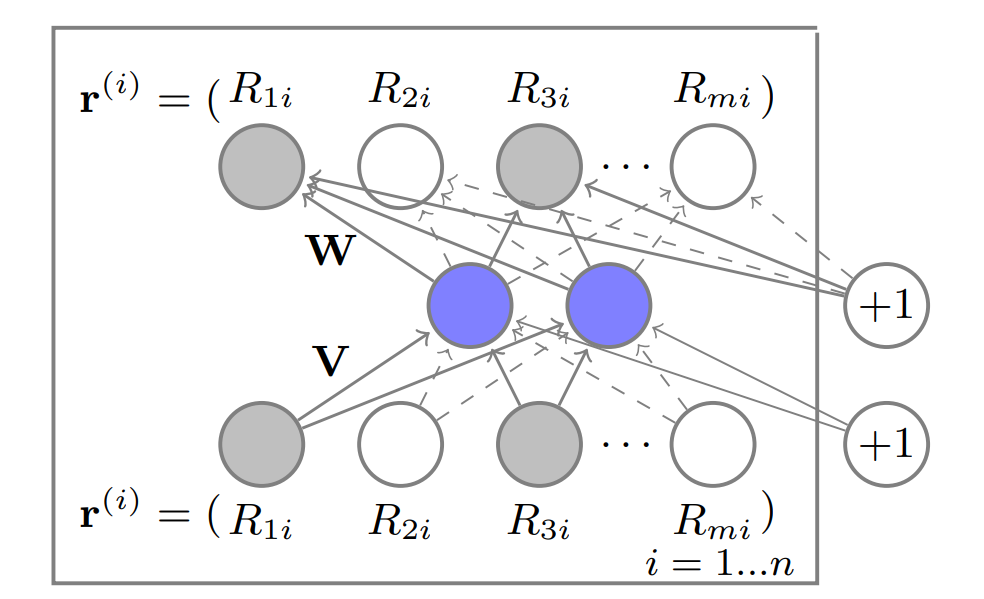
\includegraphics[width=0.5\textwidth]{figures/autorec.png}
\caption{AutoRec model architecture.}
\label{fig:autorec}
\end{figure}

\subsubsection{AutoRec model performance}
\begin{figure}[h]
	\centering
	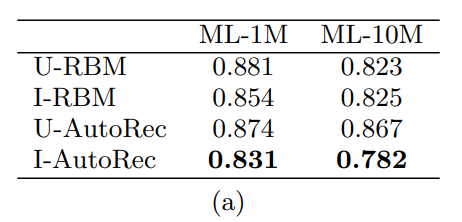
\includegraphics[width=0.3\textwidth]{figures/autorecresults1.png}\\
	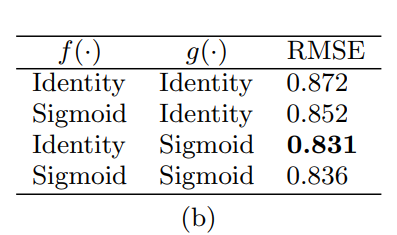
\includegraphics[width=0.3\textwidth]{figures/autorecresults2.png}\\
	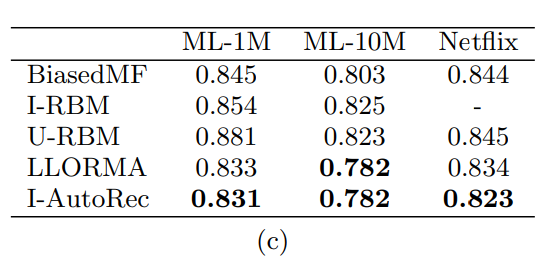
\includegraphics[width=0.3\textwidth]{figures/autorecresults3.png}
	\caption{Comparison RMSE of AutoRec and other models on different datasets.}	
	\label{fig:autorec_performance}
\end{figure}

\FloatBarrier
\subsection{Caser}
\subsubsection{User behaviour visualization discussed in Caser paper}
In the Caser paper, the authors argue that previous Markov Chain-based models fails to capture the union-level influences and skip behaviours. 
\begin{figure}[h]
\centering
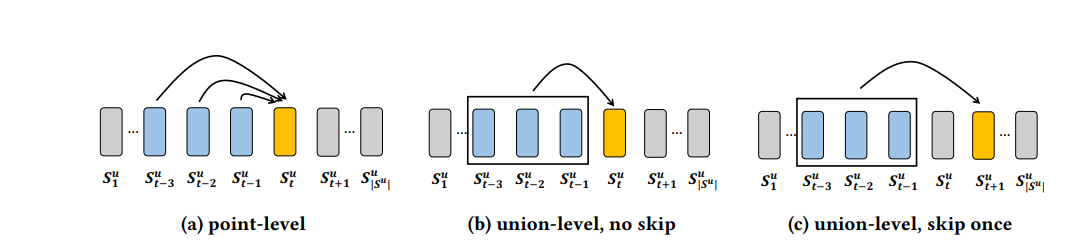
\includegraphics[width=0.5\textwidth]{figures/caser-behaviour.png}
\caption{Visualization of point-level, union-level, and skip behaviours.}
\label{fig:caser-behaviour}
\label{fig:caser1}
\end{figure}

\subsubsection{Caser model architecture}
\label{sec: caser-architecture}

The Caser model architecture is shown in figure \ref{fig:caser-architecture}. The model takes the user-item interaction matrix as input and applies horizontal and vertical convolutional filters to capture point-level and union-level interactions. The latent representation of the item-sequence is then concatenated with the user-embedding. The output of the model is a probability distribution over the items, which represents the probability of the user interacting with the item at the timestep we are predicting for.
\begin{figure}[h]
\centering
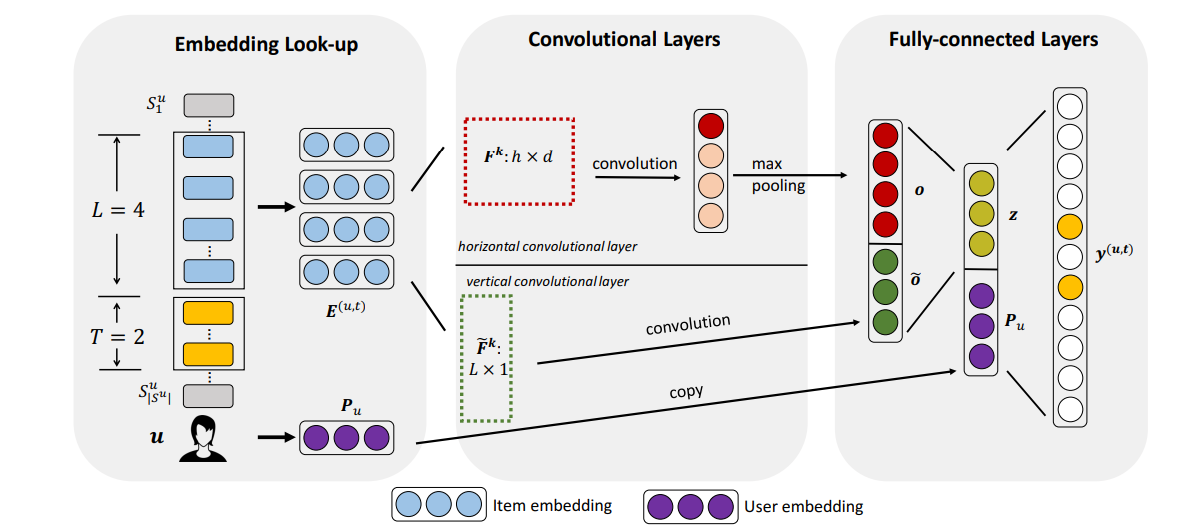
\includegraphics[width=0.5\textwidth]{figures/caser-architecture.png}
\caption{Caser model architecture.}
\label{fig:caser-architecture}
\end{figure}

\subsubsection{Caser model performance}
\begin{figure}[h]
	\centering
	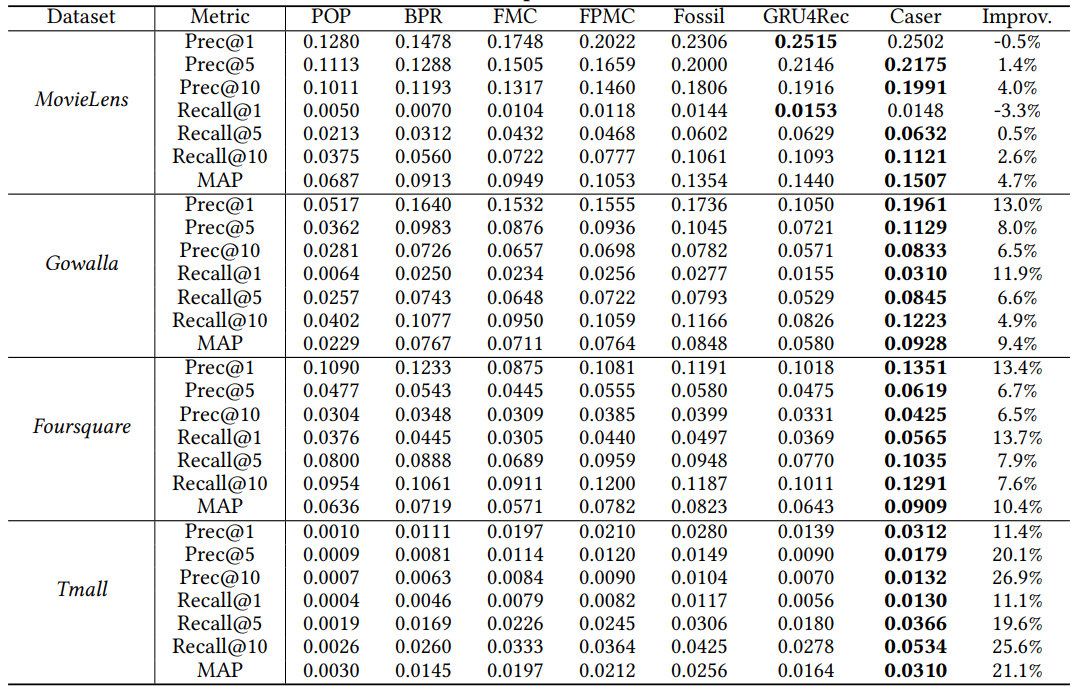
\includegraphics[width=0.5\textwidth]{figures/caser-performance.png}
	\caption{Comparison of Caser and other models on different datasets.}
	\label{fig:caser-architecture}
\end{figure}
\FloatBarrier

\subsection{RNN}
\subsubsection{RNN model architecture}
\begin{figure}[h]
\centering
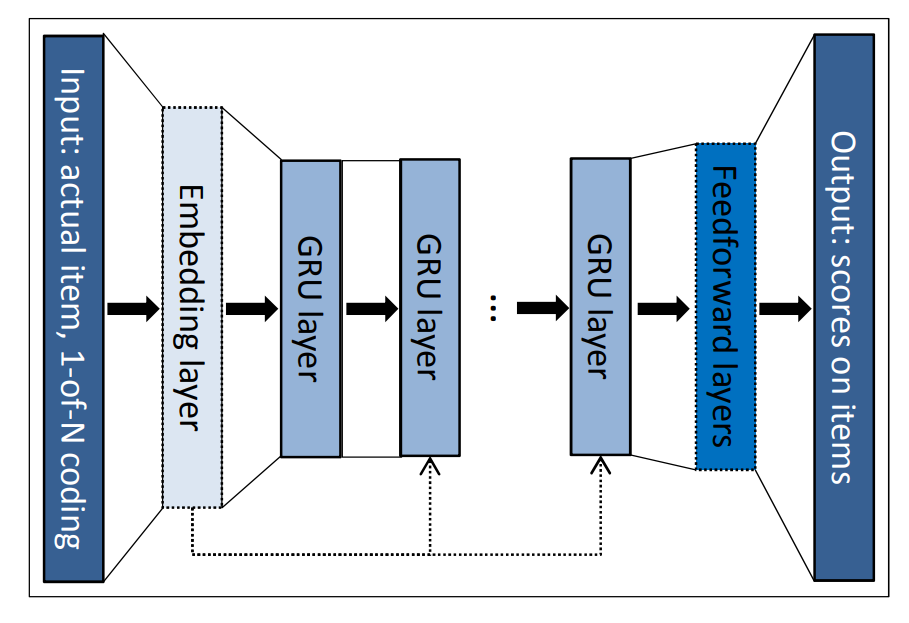
\includegraphics[width=0.5\textwidth]{figures/rnn-architecture.png}
\caption{RNN model architecture.}
\label{fig:rnn}
\end{figure}






\end{document}
